
The accuracy of the resampling process depends lagely on two user-controlled properties:

\begin{itemize}
    \item The amount of smoothing applied to continuous metadata in the corpus.  Since values are selected from the smoothed corpus values, it is possible to select values that are non-identical to the input corpus.  This is generally a desirable property, and the kernel function used to smooth the input data is user-defined and has known statistical properties.
    \item The number of documents selected.  As this increases, the overall distribution of the output corpus converges to that of the corpus description file.
\end{itemize}


The intricacy of the input distribution largely defines the necessary size of the input corpus: an input corpus that is defined only in terms of simple marginal distributions is simpler to reproduce, that is it contains \textit{less information}, than one built using the full conditional distribution of a large, general corpus such as the BNC.

The question of when to stop sampling documents is related to the problem of corpus size in general: the output corpus is conceptually a model of the input corpus, and should contain enough data to be representative of the relationships therein whilst following the same guide.  This is best assessed by measuring the uniformity of residuals.  A suitable end condition for many uses of the output would thus be a combination of corpus size and residual uniformity (notably it is possible to constantly balance the uniformity of residuals during the rejection sampling phase too).

The evaluation here establishes the resampling algorithms' ability to produce copies of the input corpus with uniform residuals, and establishes a 'best case' baseline against which the results of document retrieval may be compared.

The research questions answered by the analysis here run to:

\begin{enumerate}
    \item Does the resampler converge on the same distribution as its input?
    \item How many `target' documents are required to converge upon the input distribution (at some known probability)
\end{enumerate}


\subsection{Method}
Evaluation of the selection method is possible separately to document retrieval as the input distribution is known.  This means that, unlike a bootstrapping operation, we can rely on model deviance measures (rather than heuristics such as autocorrelation) to indicate the point at which we have sufficient data to represent the input distribution.  Since documents are retrieved and compared against their `target' as selected by this process, it is thus possible to guarantee conformance to some property of the input distribution, providing retrieval is performed accurately.  The eventual error for the corpus is a sum of these two deviances.


\begin{figure}[Ht]
    \centering
    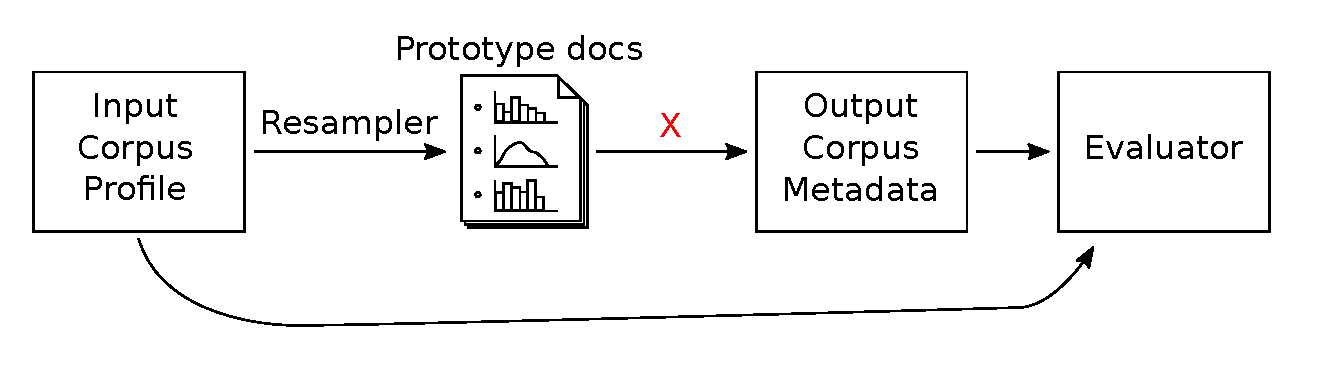
\includegraphics[width=0.9\textwidth]{evaluation/resample-overview}
    \caption{Data flow for evaluation of the sampler.}
    \label{fig:evaluation:resampling:overview}
\end{figure}


The data flow outlined in Figure~\ref{fig:evaluation:resampling:overview} is identical to that used for the final selection, with the omission of a retrieval stage at \textsl{\color{red} x}.  This means the evaluation will be performed under the assumption that the retrieval process is always able to find a suitable document.  The operation performed by the evaluator is essentially a comparison between two distributions, and may be performed using any number of algorithms with the one requirement being that it can practically be executed after each document is retrieved (note that for the purposes of this evaluation, such a requirement is less critical).

Evaluation methods provided in the prototype implementation are:

\begin{itemizeTitle}

    \item[Mean Error] For each dimension, the sum of the deviance from each document to its target value is divided by the number of documents in the collection.  This provides an asymmetric form of the commonly-used Mean Squared Error.
    \item[Distribution Comparison] A commonly used method for comparing empirical distributions, this is computed by taking the differences between the cumulative density of each dimension's data and is thus less sensitive to order than MSE methods.  Typically these methods are able to provide confidence bounds related to statistical significance.
    \item[Linear Modelling] A linear model is constructed and fit with parameters according to the input dimensions.  If this model proves statistically equivalent to the null model, then the residuals are considered uniform.

\end{itemizeTitle}


For the purposes of this evaluation, a distribution comparison method, Log-likelihood, was selected due to its known statistical bounds and wide use in corpus linguistics\footnote{It it worth noting that the log-likelihood statistic is just one of a large number of valid goodness-of-fit tests, the main contender being two-sample Kolmogorov-Smirnov}.  The major disadvantage of using this method, that it is harder to directly relate to the content of each text, is not relevant at this stage of analysis.


Log likelihood comparison methods are already widely used in corpus linguistics for keywording and corpus comparison, and have the notable property of measuring significance (using Wilks' theorem), rather than effect size (as with many information-theory-based deviance measures such as MI and Jaccard).  This evaluation makes use of such properties in that we desire to know at what point the output distribution is, to a given standard of probability, the same as the input: as we do not control the size of the input distribution we are unable to control the ultimate power of the test and thus the effect size.

This comparison of the output and input distributions was repeated as documents are re-sampled, the point at which the two cease to be significantly different noted.  This process should establish both RQs:

\begin{enumerate}
    \item Load input corpus;
    \item Repeatedly sample from the input corpus, inserting documents into the output corpus;
    \item After each document, compare the output distribution to the input.
\end{enumerate}


Note that this method treats each metadata dimension of the input corpus as an independent distribution, effectively evaluating the joint distribution of the sample.  This was done to permit comparison where obtaining a sample large enough to provide sufficient statistical power is largely impossible --- even in the BNC, there are seldom many documents that share \textsl{all} metadata values.  This has the effect of weakening the test such that the `Conditional' sampler is indistinguishable from the `Marginal' sampler (as mentioned in Section~\ref{sec:rebuilding:method:retrieval:resampling}).



\subsection{Results}

The evaluation here focuses on categorical values with over five members due to the asymptotic nature of the log-likelihood statistic making it unreliable below this number.  As such, we bin the word count into 17 bins, and use the true BNC readability category rather than the (continuous) Fleisch reading ease score.  This results in three variables that must converge prior to similarity being determined:

\begin{itemizeTitle}
    \item[Genre]  The genre category, as fit using the classifier heuristic mentioned elsewhere, only using all 70 categories;
    \item[Words]  The word count, binned to form bins with no fewer than five texts in each;
    \item[AudLvl] Audience level, categorised as `high', `med', and `low';
    \item[Mode]   \textbf{S}poken or \textbf{W}ritten.
\end{itemizeTitle}

The word count is binned irregularly due to the low frequency of files with more than 80,000 words listed in the index.  This results in a distribution shown by the historgram in Figure~\ref{fig:evaluation:resampling:bncwordhist}, with the minimum bin frequency being 8.  Other variables were left unmodified.


\begin{figure}[Ht]
    \centering
    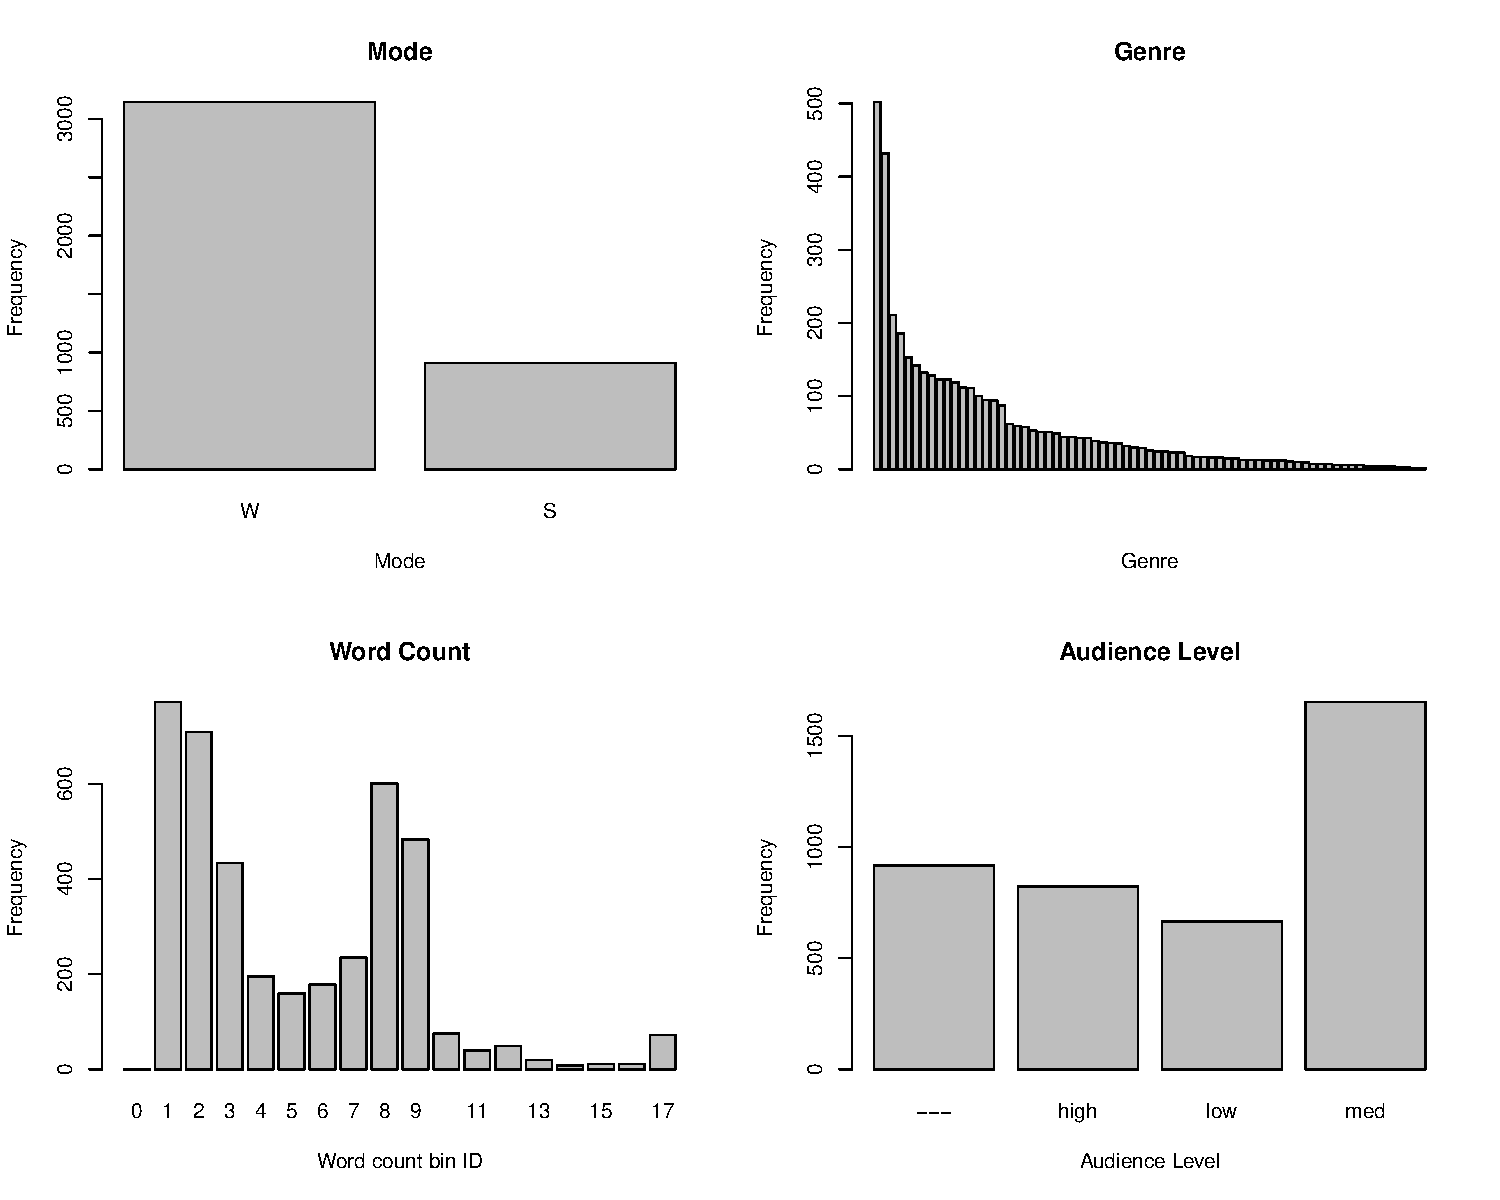
\includegraphics[width=1\textwidth]{evaluation/4waybnchist}
    \caption{Word count distribution from the BNC index (n=4054, breaks at 5k < 80k, max=428248)}
    \label{fig:evaluation:resampling:bncwordhist}
\end{figure}


The convergeance rate of each of the variables is, as mentioned above, dependent on the information content of the input bins' frequencies (due to the complexity of the sample) and the number of bins with fewer than five members (due to log-likelihood converging slowly to the $\chi^2$ distribution).  Each variable's convergeance may thus be appropriately expressed in terms of how long the average bootstrapping process takes to converge upon the distribution to a given confidence value, relative to the size of the input.

A basic description of the bins used for each input metadata item is presented in Table~\ref{table:evaluation:resampling:inputdist}.  Medians and interquartile ranges were used as centrality and deviance measures due to the Zipfian nature of the bin distributions (a feature expected to manifest in most corpora).  The `ID' column gives the `index of dispersion' --- a normalised measure of the variability in the distribution's bins computed by dividing the centrality measure (median) by the centrality measure (median).

% TODO: table with variable, bin count, num<10, stdev, mean, convergeance mean, convergeance confint@95%
\begin{table}[Ht]
    \centering

    \begin{tabular}{ |l|c|c|c|c|c| }
        \hline
        Metadata & bins & $|n_{bin} < 10|$ & $median(n_{bin})$ & $IQR(n_{bin})$ & ID  \\
        \hline
        Genre & 71  & 16 (22.5\%)   & 26    & 49        & 1.88    \\
        Words & 18  & 2 (11.1\%)    & 117.5 & 359.25    & 3.05    \\
        AudLvl& 4   & 0 (0\%)       & 869   & 317.5     & 0.36    \\
        Mode  & 2   & 0 (0\%)       & 2027  & 1117      & 0.55    \\
        \hline
    \end{tabular}
    \caption{Distributions of metadata dimensions in the input corpus (BNC index)}
    \label{table:evaluation:resampling:inputdist}
\end{table}

The figures in Table~\ref{table:evaluation:resampling:inputdist} represent common cases for real-world corpora:

\begin{itemize}
    \item `Mode' is a simple binary classification with very different group sizes.
    \item `AudLvl' is a simple classification with a very `flat' distribution.
    \item `Words' is a bimodally distributed measure with a large amount of variation but also very large numbers in each bin.  This is a good representation of the counts of many linguistic features.
    \item `Genre' is moderately heterogenous, yet has a distribution with many low-frequency items in it.
\end{itemize}

We may reason from the index of dispersion that convergeance will occur faster for `AudLvl' and `Mode' than for `Genre' and `Words' --- the ordering of the other two largely being determined by the conservative estimation of log-likelihood for low-frequency bins.


\begin{figure}[Ht]
    % ./analysis/loglik-significance.r
    \centering
    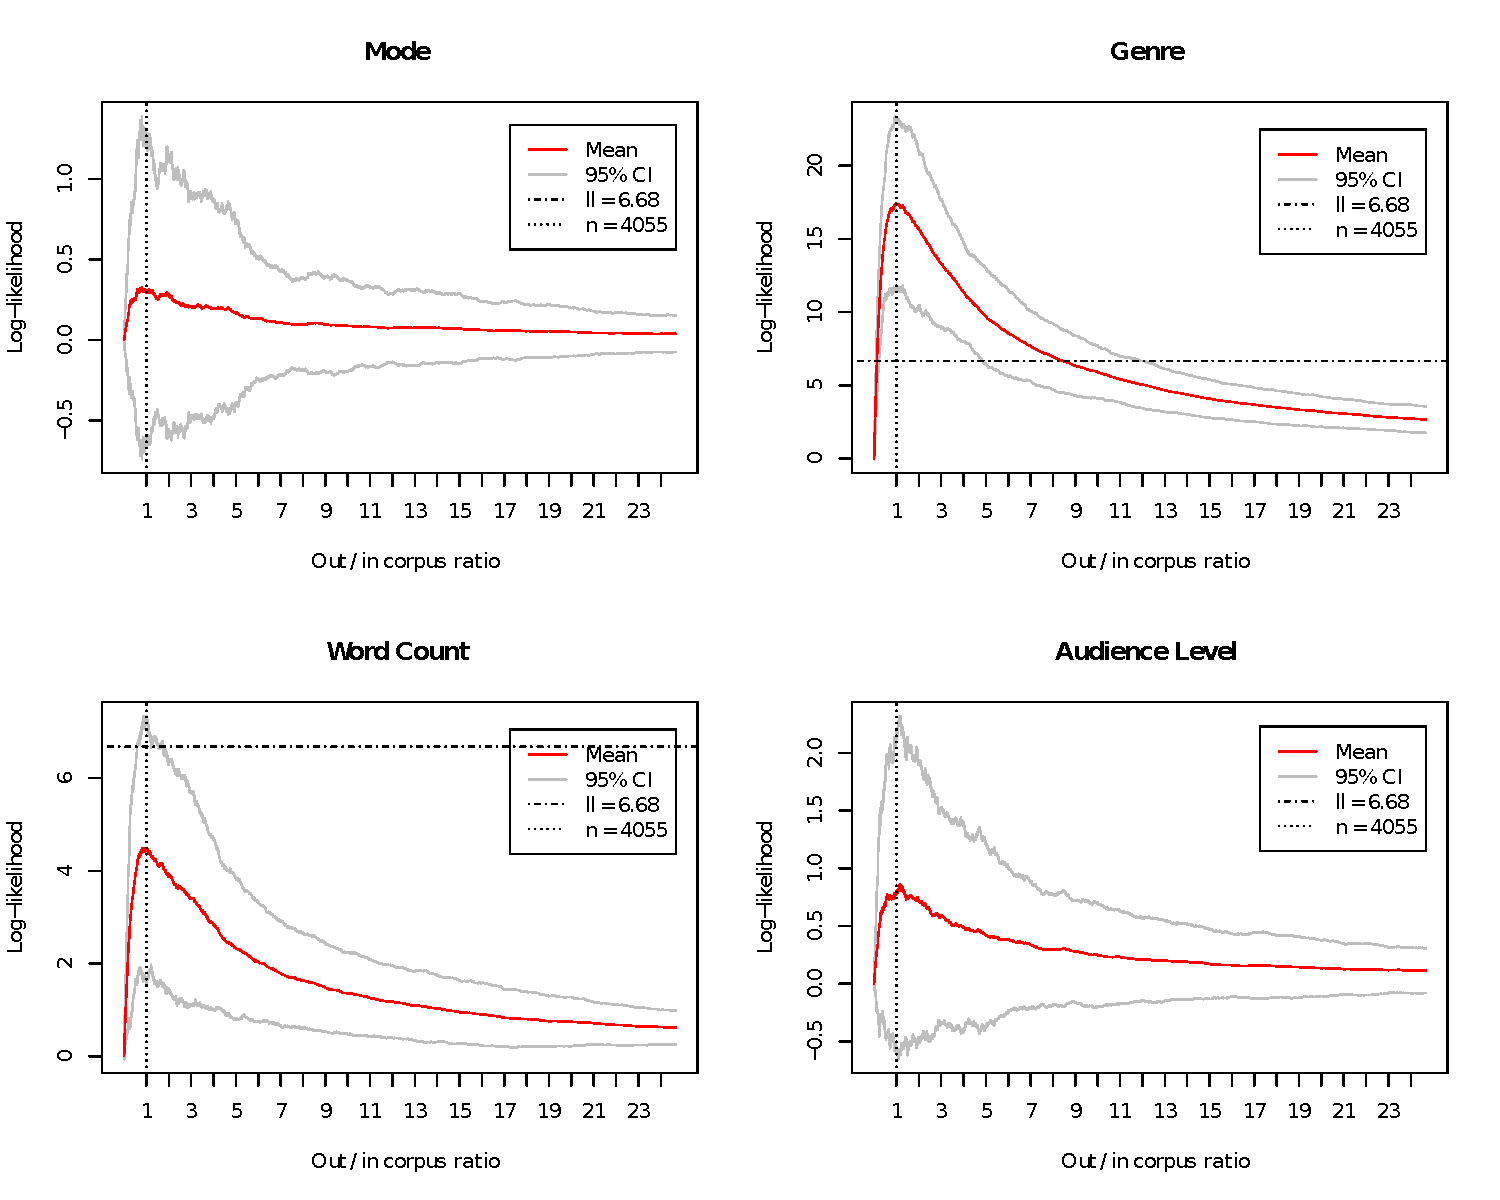
\includegraphics[width=1\textwidth]{evaluation/4wayCI95}
    \caption{Log-likelihood scores and 95\% confidence intervals for each metadata property during resampling (100 repetitions of 100,000 documents)}
    \label{fig:evaluation:resampling:4wayCI95}
\end{figure}


Figure~\ref{fig:evaluation:resampling:4wayCI95} displays the log-likelihood score of the output distribution as it is built.  These graphs clearly illustrate the relative complexity of the input distributions, as well as the downsides of estimating log-likelihood measures for low-frequency results.  After an initial burn-in period (the end of which is marked when the output distribution size matches that of the input), all dimensions gradually converge upon the target distribution.  For any input distribution with low counts, the similarity measure will not be accurate until these lowest bins are filled---marked on the graph roughly as the point where the output distribution is equal in size to the input\td{though this is not entirely precise and I think is estimable using binomial}.

The two simpler distributions, `Mode' and 'AudLvl', peak at levels well below the 95\% threshold chosen for the log-likelihood statistic.  In the case where the `target' input distribution is defined by profiling an existing corpus, this implies that we could properly build a corpus \textit{smaller} than the input (though unfortunately this is not rigorous without also know the relationship of the original input corpus to the population as it is itself generated from that sample).  The relatively confident estimates for these parameters at a 1:1 input:output ratio backs up the rational expectation that large numbers of documents in few bins will be easy to replicate.

A marginally more complex distribution of metadata in the form of the `Words' dimension shows, again, fast convergeance, requiring an output distribution roughly twice the output to replicate with 97.5\% confidence.

By far the most complex input data, `Genre', takes much longer to converge, requiring a ratio of roughly 12:1.  This result is largely a function of the low bin frequencies and the large proportion of bins that have values below the threshold at which log-likelihood may be relied upon to provide a moderately-conservative estimate.

The speed of convergeance reflects the variability that is permitted in any subsequent retrieval process: fixing the `Mode', for example, will lead to a corpus with known proportions of spoken and written text, but variability otherwise according to the population from which they are sourced.  If a particularly large corpus is available with a desirable sample design, restricting only one dimension merely refines the original sample\footnote{Of course, such a situation is difficult if the corpus from which documents are not tagged with relevant metadata, something unlikely if that dimension was not already in the sample design}.

\paragraph{}

The process of random resampling detailed here is in many ways uninteresting: after all, the experiment detailed above merely selects items based upon existing metadata.  The value in the above technique lies in its mode of use:

\begin{itemize}
    \item The distribution converged upon is arbitrary, and may be defined in the absence of an input corpus (or as a modification thereof).  This allows relaxation of a corpus description's requirements to reduce the necessary oversampling ratio above, or the addition of specific metadata items where the source of documents is particularly easy to sample according to certain properties.
    \item Halting the resampling process at any stage, due to the random selection method used, leads to an unbiased output corpus (though it may well be imprecise to the point of irrelevance).
    \item After resampling of candidate documents through a process of resampling (which has known bounds of error), the process of retrieving documents can be compared against a gold standard.
    \item When starting with a manually-designed corpus (which has bin sizes only relevant to one another), convergeance can only be achieved where the output corpus size is greater than or equal to that of the input corpus\td{I can do this experimentally by varying n for the same distribution.  It should converge at the same absolute 'n'.  Might be worth testing?}.  Aside from fitting issues where bin sizes are small, corpora fit using the same distribution shape should converge at the same size (i.e. \textsl{not} relative to the input corpus size).
\end{itemize}


% TODO: Experiment on convergion point by input n, and/or autocorrelation
% linear models for each, comment on confidence



% ---------









\til{integrate the below better, it was written standalone.}


The relationship described by the log-likelihood scores of the two corpora describes the confidence one may have in the original, input, corpus: an input corpus with very few documents in each `bin' is less powerful when used to answer questions using data in that bin, and so will require a greater number of documents in the output corpus to achieve confidence at the same effect size.  This is a useful heuristic, as it ensures that samples are never output that are not in some way large enough to be confident about their distribution, thus enforcing a minimum sample size.  Unfortunately, if this comparison is based on duplication of an existing sample (such as in this case) such an adjustment is non-rigorous as it is based upon the sample parameters, which have an unknown relationship to the population parameters they estimate.  Essentially, whilst this is a heuristic indicating internal validity, it does not ensure external validity.

A notable property of the resampler is that, even if the confidence of the output corpus being 'converged' to a given confidence level is very low (i.e. the log-likelihood score is above a given threshold), the output corpus is unbiased relative to its input due to random selection.  In addition, the convergeance of a corpus with a simpler design than the source corpus will occur at a number of documents lower than that of the input corpus, making it possible to resample an existing corpus using a design with \textit{simpler} metadata properties.  In this case, the `simplicity' of the design is defined by the information in the design distribution relative to the information content of the source corpus.  For example, if our experiment did not care about genre, it would be possible to sample texts directly from word count and audience level, producing a corpus with a mere \td{n} nexts in with a \td{n\%} confidence of representing the input corpus.






\begin{lstlisting}
example of running the thing:

Loading profile...
[genre] Loading classifier data from memdump: ./resources/list_classifier_dump.dat...
Loading corpus from /tmp/test.corpus...
Building sampler for corpus #<Corpus:3:269543840>...
Using full conditional sampling with Z = 1.645, sd = 30
Creating (virtual) output corpus...
Corpus created using 3 dimensions of metadata:
  - GENRE of type #<Impute::DiscreteDistribution:0x000000025d2710>
  - Word Total of type #<Impute::SmoothedGaussianDistribution:0x000000025d26c0>
  - Aud Level of type #<Impute::DiscreteDistribution:0x000000025d2648>
Selecting random document from #<Corpus:3:269543840>...
 - dims: 3, docs: 4054
 - dims: 2, docs: 4 (Word Total == 32528.538691473)
 - dims: 1, docs: 1 (Aud Level == low)
=> #<Impute::Document:0x0000002123f3b8
 @dimensions={"Word Total"=>32528.538691473, "Aud Level"=>"low", "GENRE"=>"W_pop_lore"},
 @id="115f72d0-94cc-4c4d-91d1-6b8cbe18a081",
 @meta={},
 @text="">
\end{lstlisting}




